\videotitle{Multi-fidelity Bayesian optimization}
%----------------------------------------------------------------------

\begin{frame}[c]{Motivating example}

\begin{itemize}
    % \item Traditional Bayesian hyperparamter optimizers model \\ the loss of ML algorithm given the dataset and seek to find \\ the minimum of such black-box function.
    % \item \emph{FABOLAS} models the loss and computational cost \\ \alert{across dataset size} and carries BO with an extra degree of freedom.
    \item Performance of an SVM on MNIST and subsets of it:\\~\\
	    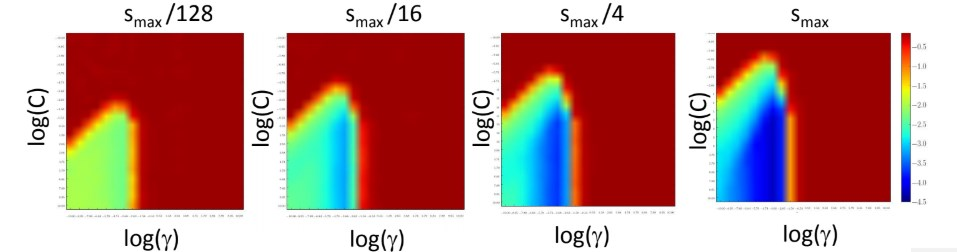
\includegraphics[width=0.9\textwidth]{../w07_hpo_speedup/images/fabolas/example_mnist.jpg}
	    \begin{itemize}
            \item Computational cost grows quadratically in dataset size $z$
            \item Error shrinks smoothly with $z$
        \end{itemize}
	\item Evaluations on the smallest subset (about 400 data points) cost 10\,000$\times$ less than on the full data set
    
\end{itemize}
\end{frame}
%----------------------------------------------------------------------
%----------------------------------------------------------------------

%----------------------------------------------------------------------
%----------------------------------------------------------------------
\begin{frame}[c]{Idea of Multi-fidelity Bayesian optimization \litw{\href{http://proceedings.mlr.press/v70/kandasamy17a.html}{Kandasamy et al, 2017}} \litw{\href{http://proceedings.mlr.press/v54/klein17a.html}{Klein et al, 2017}}}
% https://papers.nips.cc/paper/6118-gaussian-process-bandit-optimisation-with-multi-fidelity-evaluations

\begin{itemize}
	\item Recall: standard Bayesian optimization uses a model $\surro(\conf) \approx y$ to select the next $\conf$
\pause
\medskip
	\item \alert{Multi-fidelity} Bayesian optimization uses a model $\surro(\conf\alert{, z}) \approx y$ to select the next $(\conf\alert{, z})$
	\myit{
		\item Here, $z\in \mathcal{Z}$ is the fidelity; $\mathcal{Z}$ is the fidelity space, e.g., $\mathcal{Z} = [1, N_{\bullet}] \times  [1, T_{\bullet}]$
	}	 
    \pause
    \bigskip
	
%	\item BOCA - a general approach
%	\begin{itemize}
%	    \item Introduces continuity in fidelity space
%		\item Based on \alert{UCB}
%	\end{itemize}
%   
%	\item FABOLAS - a Gaussian process for extrapolating from small to large datasets
%	\begin{itemize}
%		\item This approach uses dataset size as a fidelity $(z \in [0, 1])$
%		\item Based on \alert{Entropy Search}
%	\end{itemize}


    \item Denoting $\alert{z_{\bullet}}$ as the maximum fidelity (e.g., $z_{\bullet} = [N_{\bullet},T_{\bullet}]$), our goal is to find:
        \begin{equation*}
            \optconf = \argmin_{\conf \in \pcs} \func(\conf) = \argmin_{\conf \in \pcs} \surro(\conf, \alert{z_{\bullet}})
        \end{equation*}

    \pause
    \bigskip

    \item Implications for Bayesian optimization
    \myit{
    	\item Model $\surro$ needs to be good at \alert{extrapolating} from small to large $z$
		\item Acquisition function now also needs to select $z$ (i.e., take into account cost of evaluations)
	}
\end{itemize}




\end{frame}
%----------------------------------------------------------------------
%----------------------------------------------------------------------

%----------------------------------------------------------------------
%----------------------------------------------------------------------
%\begin{frame}[c]{Bayesian Optimization with Continuous Approximations}
%
%\begin{itemize}
%    \item \emph{Goal.} Use the cheap approximations to guide search for the optimum of $\func$, \\ reduce the overall cost of optimization
%    \item \emph{Example.} Tuning of a classification algorithm over a space of hyperparameters $\conf$ 
%        \begin{itemize}
%            \item using $N_{\bullet}$ data points
%            \item via iterative algorithm for $T_{\bullet}$ iterations
%        \end{itemize}
%    \item \emph{Solution.} Approximate validation loss using fewer data points $N < N_{\bullet}$ and/or fewer iterations $T < T_{\bullet}$, such that search deploys:
%        \begin{itemize}
%            \item cheap low fidelity experiments with small $(N, T)$ to discard bad hyperparameters 
%            \item expensive high fidelity experiments with large $(N, T)$ for promising regions
%        \end{itemize}
%    
%\end{itemize}
%\end{frame}
%----------------------------------------------------------------------
%----------------------------------------------------------------------

%----------------------------------------------------------------------
%----------------------------------------------------------------------
%\begin{frame}[c]{Bayesian Optimization with Continuous Approximations}
%
%\begin{itemize}
%
%        \begin{itemize}
%            \item surrogate function $\surro : \alert{\mathcal{Z}} \times \conf \rightarrow  \mathbb{R}$
%            \item e.g. fidelity space $\mathcal{Z} = [1, N_{\bullet}] \times  [1, T_{\bullet}], z_{\bullet} = [N_{\bullet}, T_{\bullet}]$
%
%        \end{itemize}
%
%    \item Determine the fidelity $\iter[\bocount]{z} \in \mathcal{Z}$ to query $\surro$:
%        \begin{enumerate}
%            \item Select a subset  $\iter[\bocount]{Z}$ of $\mathcal{Z}$, that:
%                \begin{itemize}
%                    \item considers only cheaper fidelities,
%                    \item trades of \emph{information gain} and \emph{cost} while enforcing more exploration \\ in cheaper regions in the early stage of the search, %
%                    \item excludes fidelities in a close neighborhood of $z_{\bullet}$.
%                \end{itemize}
%            \item If the subset is empty: $\iter[\bocount]{z} = z_{\bullet}$
%            \item Otherwise: $\iter[\bocount]{z} \in \argmin_{z \in \iter[\bocount]{Z}} \cost(z)$
%        \end{enumerate}
%
%\end{itemize}
%\end{frame}
%----------------------------------------------------------------------
%----------------------------------------------------------------------

% %----------------------------------------------------------------------
% %----------------------------------------------------------------------
% \begin{frame}[c]{Fast Bayesian Optimization on Large Datasets}
% \framesubtitle{Multi-fidelity Bayesian optimization}

% \alert{Multi-fidelity Bayesian optimization} for fidelity with values $z\in \mathcal{Z}$ 
% \begin{itemize}
% 	\item Standard Bayesian optimization uses a model $\func(\conf) \approx y$ to select the next $\conf$
% 	\item \alert{Multi-fidelity Bayesian optimization} uses a model $\func(\conf\alert{, z}) \approx y$ to select the next $(\conf\alert{, z})$
%     \pause
%     \smallskip
    
% 	\item Model $\func$ needs to be good at extrapolating from small to large $z$
	
% 	\item E.g., a Gaussian process for extrapolating from small to large datasets - FABOLAS
% 	\begin{itemize}
% 		\item This approach uses dataset size as a fidelity $(z \in [0, 1])$,
% 		\item based on \alert{Entropy Search},
% 		\item achieved 1\,000-fold speedups for SVM on MNIST example.
% 	\end{itemize}
% \end{itemize}
% \end{frame}
% %----------------------------------------------------------------------
% %----------------------------------------------------------------------

%----------------------------------------------------------------------
%----------------------------------------------------------------------
\begin{frame}[c]{Entropy Search: Reminder}

\begin{itemize}
		\item Define the $p_{\text{min}}$ distribution given data $\dataset$:
		$$p_{\text{min}}(\conf^* \mid \alert{\dataset}) := p(\conf^* \in \argmin_{\conf\in \pcs} \func(\conf) \mid \alert{\dataset})$$
	
		\item Entropy search \lit{\href{http://jmlr.csail.mit.edu/papers/volume13/hennig12a/hennig12a.pdf}{Hennig et al. 2012}} aims to minimize the entropy \alert{$\mathcal{H}[p_\text{min}]$}
		\myit{
			\item It aims to be maximally certain about the location of $\conf^*$
		}
\bigskip
\pause
		\item In a nutshell: select 
%		\begin{enumerate}
%			\item Estimate $p(\func \mid \dataset)$, e.g., using a GP 
%			\item Approximate $p_\text{min}$ by representer points and Monte-Carlo simulations
%			\item Select 
$\conf$ that maximizes the following acquisition function:
%		\end{enumerate}
\end{itemize}
\vspace*{0.5cm}
	\[{\acq}_{ES}(\conf) := \mathcal{H}[p_{\text{min}}(\cdot \mid \alert{\dataset})] - \mathds{E}_{\alert{p(\tilde{\cost}\mid \conf, \dataset)}} 
	\left[   \mathcal{H}[p_{\text{min}}(\cdot \mid \alert{\dataset \cup \left\langle \conf, \tilde{\cost} \right\rangle })] \right]\]

\end{frame}
%----------------------------------------------------------------------
%----------------------------------------------------------------------

%----------------------------------------------------------------------
%----------------------------------------------------------------------
\begin{frame}[c]{Entropy Search for Multi-Fidelity Optimization \litw{\href{http://proceedings.mlr.press/v54/klein17a/klein17a.pdf}{Klein, Falkner \& Hutter, 2017}}}

\begin{itemize}
		\item We now care about the $p_{\text{min}}$ distribution for the maximal budget $z_{\bullet}$:
		$$p_{\text{min}}(\conf^* \mid \dataset) := p(\conf^* \in \argmin_{\conf\in \pcs} \func(\conf\alert{,z_{\bullet}}) \mid \dataset)$$
	
		\item We still want to minimize the entropy $\mathcal{H}[p_\text{min}]$
\pause
\medskip
		\item Now we aim for the biggest \alert{reduction in entropy per time spent}
		\begin{itemize}
			\item Now we don't model only $\func$, but also \alert{the cost $c(\conf,z)$}
			\item We choose the next $(\conf,z)$ by maximizing:
		\end{itemize}
\end{itemize}
\vspace*{0.5cm}
	\[{\acq}_{ES}(\conf,z \mid \dataset) := \mathds{E}_{\alert{p(\tilde{\cost}\mid (\conf, z), \dataset)}} 
	\left[   \frac{\mathcal{H}[p_{\text{min}}(\cdot \mid \alert{\dataset})] - \mathcal{H}[p_{\text{min}}(\cdot \mid \alert{\dataset \cup \left\langle (\conf,z), \tilde{\cost} \right\rangle}}{\alert{c(\conf,z)}} \right]\]

%	\item Introduced to handle large datasets, in paper ``Fast Bayesian Optimization on Large Datasets (Fabolas)'' by \lit{\href{http://proceedings.mlr.press/v54/klein17a/klein17a.pdf}{Klein, Falkner \& Hutter, 2017}}

\end{frame}
%----------------------------------------------------------------------
%----------------------------------------------------------------------

%----------------------------------------------------------------------
%----------------------------------------------------------------------
\begin{frame}[c]{Entropy Search for Multi-Fidelity Optimization \litw{\href{http://proceedings.mlr.press/v54/klein17a/klein17a.pdf}{Klein, Falkner \& Hutter, 2017}}}

\begin{itemize}
    \item The entire algorithm iterates the following 2 steps until time is up:
		\begin{enumerate}
			\item Select $(\conf,z)$ by maximizing:
    			\[{\acq}_{ES}(\conf,z \mid \dataset) := \mathds{E}_{\alert{p(\tilde{\cost}\mid (\conf, z), \dataset)}} 
            	\left[   \frac{\mathcal{H}[p_{\text{min}}(\cdot \mid \alert{\dataset})] - \mathcal{H}[p_{\text{min}}(\cdot \mid \alert{\dataset \cup \left\langle (\conf,z), \tilde{\cost} \right\rangle}}{\alert{c(\conf,z)}} \right]\]
			\item Observe performance $f(\conf,z)$ and cost $c(\conf,z)$ and update models for $f$ and $c$ 
		\end{enumerate}

\pause

    \item The algorithm originally focussed on data subsets and is therefore dubbed \\ \alert{Fabolas}: 
    ``Fast Bayesian Optimization on Large Datasets''
	
\pause

\begin{columns}[T] % align columns
\begin{column}{.48\textwidth}


    \begin{block}{Advantages}
    \begin{itemize}
    	\item Conceptually beautiful
    	\item 1\,000-fold speedups for optimizing SVMs on MNIST
    \end{itemize}
    \end{block}
\pause
\end{column}%

\hfill%

\begin{column}{.48\textwidth}

    \begin{block}{Disadvantages}
    \begin{itemize}
    	\item \alert{Scalability} of GPs is a big problem (limits size of initial design)
    	\item Limited applicability of Gaussian processes
    \end{itemize}
\end{block}

\end{column}
\end{columns}   

\end{itemize}
\end{frame}
%----------------------------------------------------------------------
%----------------------------------------------------------------------


% %----------------------------------------------------------------------
% %----------------------------------------------------------------------
% \begin{frame}[c]{Fast Bayesian Optimization on Large Datasets}
% \framesubtitle{Overview}

% \begin{itemize}
%     \item Automatically choose dataset size for each evaluation
%         \begin{itemize}
%             \item Include extra dimension in probabilistic model to capture \\ dependence on dataset size $s$: $\func(\conf, s)$
%             \item Construct a second model for computational cost: $\cost(\conf, s)$
%             \item Trade off information gain about global optimum vs. cost
%         \end{itemize}
%     \item Extend the GP by an additional input dimension: $s \in [0, 1]$
%         \begin{itemize}
%             \item standard stationary kernel (over HPs) + covariance function in $s$
%                 \begin{equation*}
%                     \kernel( (\conf, s), (\conf', s') ) = \kernel_{5/2} (\conf, \conf') ( \phi^{T}(s) * \Sigma_{\phi} * \phi(s') )
%                 \end{equation*}
%             \item  we use the same form of kernel to model the loss $\func$ and cost $\cost$, but with different basis functions $\phi_{\func}$ and $\phi_{\cost}$
%                 \begin{itemize}
%                     \item $\phi_{\func}(s) = (1, (1-s)^2)^T$
%                     \item $\phi_{\cost}(s) = (1, s)^T$
%                 \end{itemize}
%         \end{itemize}
        
% \end{itemize}

% \source{Klein, Bartels, Falkner, Hennig, Hutter, AISTATS 2017}
% \end{frame}
% %----------------------------------------------------------------------
% %----------------------------------------------------------------------

%----------------------------------------------------------------------


\begin{frame}{Questions to Answer for Yourself / Discuss with Friends}

\bigskip

\begin{itemize}
    \item \alert{Discussion.} What kind of cost model would you use in Fabolas?
\medskip
	\item \alert{Discussion.} Could one use an acquisition function other than entropy search for Fabolas?    

\end{itemize}

\end{frame}